\documentclass{article}
\usepackage[landscape]{geometry}
\usepackage{url}
\usepackage{multicol}
\usepackage{amsmath}
\usepackage{esint}
\usepackage{amsfonts}
\usepackage{tikz}
\usetikzlibrary{decorations.pathmorphing}
\usepackage{amsmath,amssymb}
\usepackage{colortbl}
\usepackage{xcolor}
\usepackage{mathtools}
\usepackage{amsmath,amssymb}
\usepackage{enumitem}
\makeatletter

\newcommand*\bigcdot{\mathpalette\bigcdot@{.5}}
\newcommand*\bigcdot@[2]{\mathbin{\vcenter{\hbox{\scalebox{#2}{$\m@th#1\bullet$}}}}}
\makeatother

\usepackage[english,russian]{babel}
\usepackage[utf8]{inputenc}
\usepackage[dvips]{graphicx}
\graphicspath{{noiseimages/}}
\usepackage[unicode, pdftex]{hyperref}
\hypersetup{
  colorlinks,
  citecolor= blue,
  linkcolor = blue,
  urlcolor= blue,
}


\advance\topmargin-.8in
\advance\textheight3in
\advance\textwidth3in
\advance\oddsidemargin-1.45in
\advance\evensidemargin-1.45in
\parindent0pt
\parskip2pt
\newcommand{\hr}{\centerline{\rule{3.5in}{1pt}}}
%\colorbox[HTML]{e4e4e4}{\makebox[\textwidth-2\fboxsep][l]{texto}

\begin{document}

\begin{center}{\huge{\textbf{Основные формулы по тригонометрии}}}\\
\end{center}
\begin{multicols*}{2}

\tikzstyle{mybox} = [draw=black, fill=white, very thick,
    rectangle, rounded corners, inner sep=10pt, inner ysep=10pt]
\tikzstyle{fancytitle} =[fill=black, text=white, font=\bfseries]


\begin{tikzpicture}
\node [mybox] (box){%
    \begin{minipage}{0.46\textwidth}
    
	\begin{tabular}{lp{8cm} l}
    	Определение: 
    	& $\sin{A} = \frac{a}{c}, \cos{A} = \frac{b}{c}, \tg{A} = \frac{a}{b}, \ctg{A} = \frac{b}{a}$,\\
        & где $a$ противолежащий катет для $\angle A$,  \\
        & $b$ прилежащий катет для $\angle A$, $c$ гипотенуза \\ 

    	Из определения: & $\tg{A} \cdot \ctg{A} = 1, \tg{A} = \frac{\sin{A}}{\cos{A}}, \ctg{A} = \frac{\cos{A}}{\sin{A}}$  \\
	\end{tabular}
	
    \end{minipage}
};

\node[fancytitle, right=10pt] at (box.north west) {Определение в прямоугольном треугольнике};
\end{tikzpicture}

\begin{tikzpicture}
\node [mybox] (box){%
    \begin{minipage}{0.46\textwidth}
    
    Функции $\sin{x}, \cos{x}, \tg{x}, \ctg{x}$ вводятся через единичную окружность, \\ 
    $sin{x}$ - проекция на ось $OY$, $cos{x}$ - проекция на ось $OX$. Тангенс и котангенс также можно определить через построение.\\

    \textbf{Четность нечетность функций:} \\ 
    $\sin(-x) = -\sin(x)$ (нечетная), $\cos(-x) = \cos(x)$ (четная) \\ 
    $\tg(-x) = -\tg(x)$ (нечетная), $\ctg(-x) = -\ctg(x)$ (нечетная) 
    \end{minipage}
};

\node[fancytitle, right=10pt] at (box.north west) {Функции sinx, cosx, tgx, ctgx};
\end{tikzpicture}


\begin{tikzpicture}
\node [mybox] (box){%
    \begin{minipage}{0.46\textwidth}
  	
    \textbf{Основные формулы}:
    
    \begin{tabular}{lp{8cm} l}
    	Синус суммы: & $\sin(a + b) = \sin{a} \cdot \cos{b} + \cos{a} \cdot \sin{b}$\\
        Синус разности: & $\sin(a - b) = \sin{a} \cdot \cos{b} - \cos{a} \cdot \sin{b}$ \\
        Косинус суммы: & $\cos(a + b) = \cos{a} \cdot \cos{b} - \sin{a} \cdot \sin{b}$ \\
        Косинус разности: & $\cos(a - b) = \cos{a} \cdot \cos{b} + \sin{a} \cdot \sin{b}$ \\
    	
	\end{tabular}
    
    \textbf{Дополнительные формулы:}
    
    \begin{tabular}{lp{8cm} l}
    
    	Тангенс суммы: & $\tg(a + b) = \frac{\tg{a} + \tg{b}}{1 - \tg{a}\tg{b}}$\\

        Тангенс разности: &$\tg(a - b) = \frac{\tg{a} - \tg{b}}{1 + \tg{a}\tg{b}}$
	\end{tabular}
    \end{minipage}
};
\node[fancytitle, right=10pt] at (box.north west) {Формулы суммы и разности углов};
\end{tikzpicture}

\begin{tikzpicture}
\node [mybox] (box){%
    \begin{minipage}{0.46\textwidth}
    \textbf{Основные формулы}:
    
    \begin{tabular}{lp{8cm} l}
    	Синус двойного угла: & $\sin(2a) = 2\sin{a}\cos{a}$\\
        Косинус двойного угла: & $\cos(2a) = \cos^{2}{a} - \sin^{2}{a} = 2\cos^{2}{a} - 1 = 1 - 2\sin^{2}{a}$\\
	\end{tabular}
    
    \textbf{Дополнительные формулы:}
    
    \begin{tabular}{lp{8cm} l}
    
    	Тангенс двойного угла: & $\tg(2a) = \frac{2\tg{a}}{1 - \tg^{2}{a}}$\\
	\end{tabular}
    \end{minipage}
};
\node[fancytitle, right=10pt] at (box.north west) {Формулы двойных углов};
\end{tikzpicture}

\begin{tikzpicture}
\node [mybox] (box){%
    \begin{minipage}{0.46\textwidth}
    \textbf{Основные формулы}:
    
    \begin{tabular}{lp{8cm} l}
    	Сумма синусов: & $\sin{a} + \sin{b} = 2\sin{\frac{a + b}{2}} \cos{\frac{a - b}{2}}$\\
        Разность синусов: & $\sin{a} - \sin{b} = 2\cos{\frac{a + b}{2}} \sin{\frac{a - b}{2}}$\\
        Сумма косинусов: & $\cos{a} + \cos{b} = 2\cos{\frac{a + b}{2}} \cos{\frac{a - b}{2}}$\\
        Разность косинусов: & $\cos{a} - \cos{b} = -2\sin{\frac{a + b}{2}} \sin{\frac{a - b}{2}}$\\
	\end{tabular}
    
    \textbf{Дополнительные формулы:}
    
    \begin{tabular}{lp{8cm} l}
    
    	Сумма тангенсов: & $\tg{a} + \tg{b}  = \frac{\sin{(a + b)}}{\cos{a} \cos{b}}$\\
        Разность тангенсов: & $\tg{a} - \tg{b}  = \frac{\sin{(a - b)}}{\cos{a} \cos{b}}$
	\end{tabular}
    \end{minipage}
};
\node[fancytitle, right=10pt] at (box.north west) {Формулы суммы разности тригонометических функций};
\end{tikzpicture}


\begin{tikzpicture}
\node [mybox] (box){%
    \begin{minipage}{0.46\textwidth}
    \textbf{Основные формулы}:
    
    \begin{tabular}{lp{8cm} l}
    	Произведение синусов: & $\sin{a} \cdot \sin{b} = \frac{1}{2} \cdot (\cos (a - b) - \cos (a + b))$\\
        Произведение косинусов: & $\cos{a} \cdot \cos{b} = \frac{1}{2} \cdot (\cos (a - b) + \cos (a + b))$\\
        Произведение синуса и косинуса: & $\sin{a} \cdot \cos{b} = \frac{1}{2} \cdot (\sin (a - b) + \sin (a + b))$\\
	\end{tabular}
    
    \textbf{Дополнительные формулы:}
    
    \begin{tabular}{lp{8cm} l}
    
    	Произведение тангенсов: & $\tg{a} \cdot \tg{b} = \frac{\tg{a} + \tg{b}}{\ctg{a} + \ctg{b}}$\\
        Произведение котангенсов: & $\ctg{a} \cdot \ctg{b} = \frac{\ctg{a} + \ctg{b}}{\tg{a} + \tg{b}}$\\
	\end{tabular}
    \end{minipage}
};
\node[fancytitle, right=10pt] at (box.north west) {Произведение синусов косинусов тангенсов котангенсов};
\end{tikzpicture}

\begin{tikzpicture}
\node [mybox] (box){%
    \begin{minipage}{0.46\textwidth}
    \textbf{Основные формулы}:
    
    \begin{tabular}{lp{8cm} l}
    	Синус половинного аргумента: & $\sin^{2}{\frac{a}{2}} = \frac{1 - \cos{a}}{2}$\\
        Косинус половинного аргумента: & $\cos^{2}{\frac{a}{2}} = \frac{1 + \cos{a}}{2}$\\
	\end{tabular}
    \end{minipage}
};
\node[fancytitle, right=10pt] at (box.north west) {Формулы половинных аргументов};
\end{tikzpicture}

\textbf{Формулы приведения:}
\begin{center}
    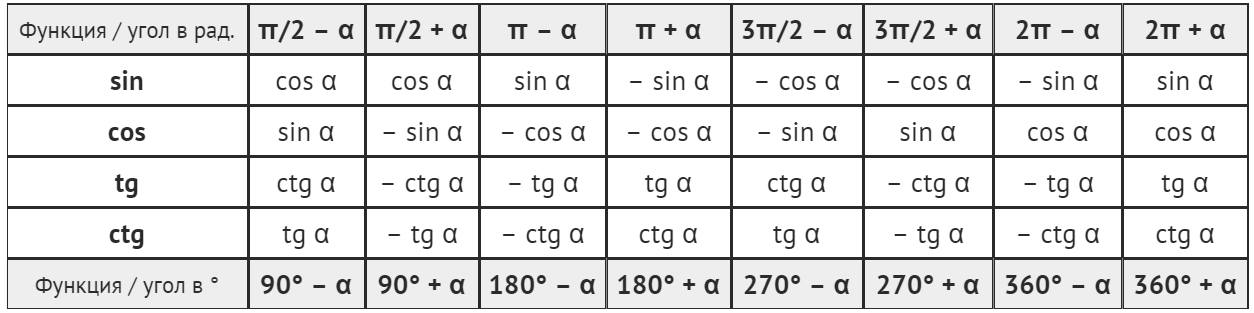
\includegraphics[keepaspectratio=true,scale=0.59]{photo1.png}
\end{center}

\textbf{Табличные значения тригонометрических функций:}
\begin{center}
    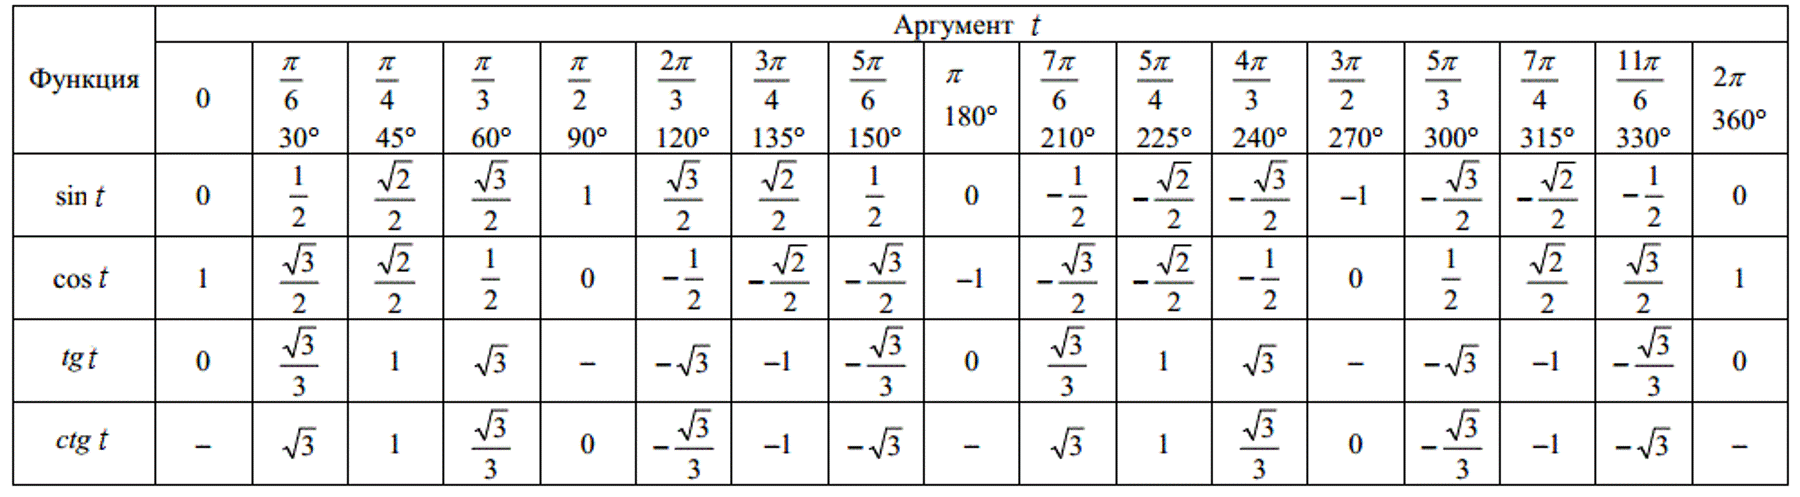
\includegraphics[keepaspectratio=true,scale=0.2056]{photo2.png}
\end{center}

\textbf{От автора:}

Этот материал поможет в структурировании формул по тригонометрии, однако важным является умение выводить большую часть этих формул. Вывод всей теории можно посмотреть на \href{https://www.youtube.com/watch?v=Jmlm2BkNUCI&t=1477s}{моем канале}. Также буду признателен, если подпишешься на мою открытую группу в Telegram: \href{https://t.me/analitiqtutor}{@analitiqtutor}, там ты сможешь найти больше материалов по математике, физике, информатике и программированию. Будем на связи.


\end{multicols*}
\end{document}
